\chapter{Resultados e discussões}

\section{Resultados do modelo GRU}
\label{sec:resultados_gru}

A seguir, os resultados alcançados pelo modelo descrita em \ref{fig:gru_pura}:

\begin{table}[H]
\centering
\caption{Resultados do GRU (\textit{N} vs. \textit{V}) na validação}
\label{tab:resultado_cv_gru_validacao}
\begin{tabular}{lcc}
\hline
\textbf{Métrica} & \textbf{Média} & \textbf{Desvio Padrão} \\
\hline
Precisão & 0.8515 & 0.1825 \\
\textit{Recall} & 0.8039  & 0.0795 \\
\textit{F1-Score} & 0.8060 & 0.0760 \\
Acurácia & 0.9640 & 0.0278 \\
\hline
\end{tabular}
\legend{Fonte: Elaborado pelo autor.}
\end{table}

Na tabela \ref{tab:resultado_cv_gru_validacao}, tem-se as métricas médias com seus respectivos desvio padrão na \textit{cross-validação} de cinco \textit{folds}.
Os resultados indicam que o modelo achou aproximadamente 80\% dos casos positivos, com um desvio padrão relativamente baixo, indicando boa estabilidade.
Além disso, a precisão do modelo foi maior que seu \textit{recall}, indicando um perfil mais conservador na classificação. 

A seguir os resultados no treino:

\begin{table}[H]
\centering
\caption{Resultados do GRU (\textit{N} vs. \textit{V}) no treino}
\label{tab:resultado_cv_gru_treino}
\begin{tabular}{lcc}
\hline
\textbf{Métrica} & \textbf{Média} & \textbf{Desvio Padrão} \\
\hline
Precisão & 0.9872 & 0.0121 \\
\textit{Recall} & 0.9782 & 0.0150 \\
F1-Score & 0.9827 & 0.0134 \\
Acurácia & 0.9969 & 0.0024 \\
\hline
\end{tabular}
\legend{Fonte: Elaborado pelo autor.}
\end{table}

Comparando os resultados da tabela \ref{tab:resultado_cv_gru_treino} com o da \ref{tab:resultado_cv_gru_validacao}, há uma evidência de sobreajuste; isto é, o modelo apresenta uma falha em sua capacidade
de generalização. Durante o treino de um modelo de aprendizado de máquina, busca-se a partir de uma amostra da população estimar uma curva que melhor
se encaixa na população. Modelos flexíveis como uma rede neural tem uma grande capacidade de se ajustar a essa amostra e, caso ela seja pequena, por exemplo,
o modelo pode acabar aprendendo as particularidades da amostra ao invés de padrões generalizáveis. 

No caso do MIT-BIH; o desbalanceamento junto com as diferenças entre os batimentos de cada paciente pode ter causado esse sobre-ajuste.

Na figura \ref{fig:gru_resultados_por_fold}, está os resultados alcançado pelo modelo em cada \textit{fold} na validação:

\begin{figure}[H]
  \centering
  \caption{Métricas do modelo \ref{fig:gru_pura} por fold \textit{fold}}
   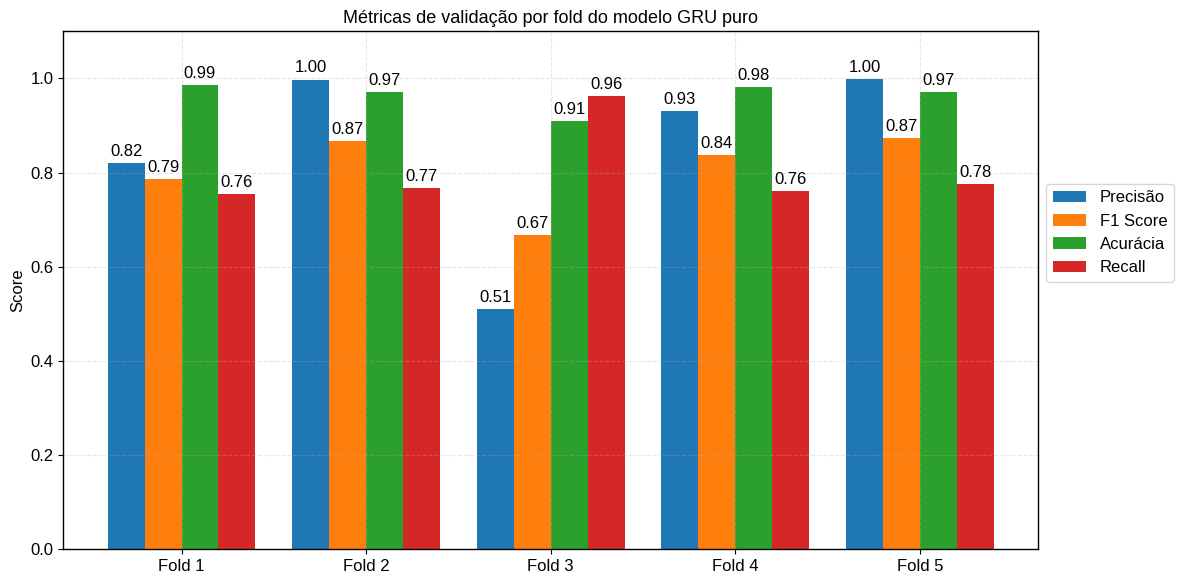
\includegraphics[width=1.0\textwidth]{figuras/modelos_resultados/gru/gru_metricas_por_fold.png} % insere o tikzpicture puro
  \label{fig:gru_resultados_por_fold}
    \legend{Fonte: Elaborado pelo autor.}
\end{figure}

No \textit{fold} três, o modelo obteve sua menor precisão, aproximadamente 0,51 porém obteve um alto \textit{recall}, aproximadamente 0,96.
Essa discrepância sugere que neste \textit{fold}, havia batimentos normais que fugiam do padrão aprendido no treino, fazendo com que o modelo
confundisse eles com batimentos da classe V. Nos demais \textit{folds}, a precisão foi maior que o \textit{recall}, sugerindo a presença 
de arritmias com características mais sutis, que fizeram com que o modelo as confundissem com batimentos normais.

Considerando o \textit{f1-score}, o terceiro \textit{fold} foi eleito o pior. Como o \textit{fold} cinco empatou com o segundo por 
esse mesmo critério, como desempate, aquele com o maior \textit{recall}, o quinto, foi considerado o melhor. 

Na figura \ref{fig:matriz_confusao_melhor_fold_gru}, está a matriz de confusão do modelo em seu melhor \textit{fold}:

\begin{figure}[H]
  \centering
  \caption{Matriz de confusão do modelo \ref{fig:gru_pura} em seu melhor \textit{fold}}
   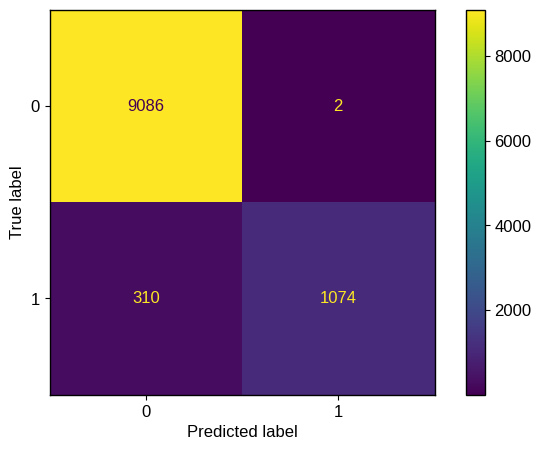
\includegraphics[width=0.7\textwidth]{figuras/modelos_resultados/gru/matriz_confusao_melhor_fold_gru_alt.png} % insere o tikzpicture puro
  \label{fig:matriz_confusao_melhor_fold_gru}
    \legend{Fonte: Elaborado pelo autor.}
\end{figure}

Na matriz, é possível ver o desbalanceamento das classes. Neste \textit{fold}, o número de sequencias pertencentes a classe
negativa é 9.088, enquanto que 1.384 pertencem a positiva; ou seja, aproximadamente, 13,21\% de todas as sequencias são
da classe positiva. 

A maioria dos erros cometidos são de falsos negativos; o modelo classificou 310 sequencias arrítmicas como normais e 
apenas duas normais como arrítmicas. Algo que já era evidenciado no gráfico \ref{fig:gru_resultados_por_fold}, pois 
sua precisão foi maior que seu \textit{recall}.

%O modelo achou 78\% das arritmias. Porém no pior, como pode ser visto na figura \ref{fig:ap_gru_pior_fold}, o modelo conseguiu achar 96\% das arritmias.
Na figura \ref{fig:matriz_confusao_pior_fold_gru}, é dada a matriz de confusão no pior \textit{fold}

\begin{figure}[H]
  \centering
  \caption{Matriz de confusão do modelo \ref{fig:gru_pura} em seu pior \textit{fold}}
   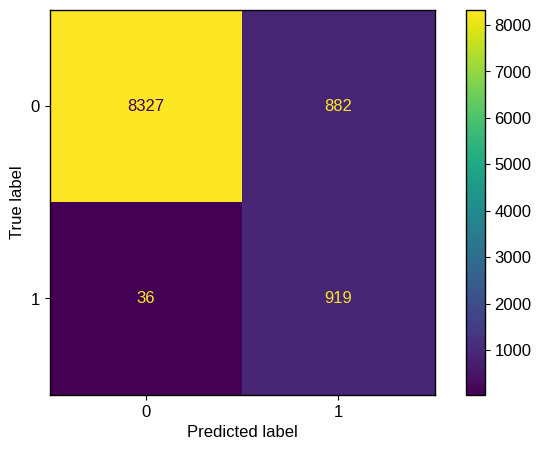
\includegraphics[width=0.7\textwidth]{figuras/modelos_resultados/gru/matriz_confusao_pior_fold_gru_alt.png} % insere o tikzpicture puro
  \label{fig:matriz_confusao_pior_fold_gru}
  \legend{Fonte: Elaborado pelo autor.}
\end{figure}

Aqui o desbalanceamento foi mais severo; havia 9.209 classes negativas e 955 classes positivas; 9,39\% aproximadamente. 
Neste \textit{fold}, a situação se inverte: a maioria dos erros foram de falsos positivos, confirmando o que foi visto no 
gráfico \ref{fig:gru_resultados_por_fold}.

%As duas figuras ilustram como o modelo conseguiu aprender melhor a classe negativa do que a classe positiva; evidenciado pelo fato dele confundir
%muito menos negativo com positivo do que o contrário. Um resultado esperado devido a essa ser a classe dominante em todos os \textit{folds}.

A seguir, na figura \ref{fig:roc_cnn_gru_melhor_fold}, a curva ROC no melhor \textit{fold}:

\begin{figure}[H]
  \centering
  \caption{Curva \textit{ROC} modelo \ref{fig:gru_pura} em seu melhor \textit{fold}}
   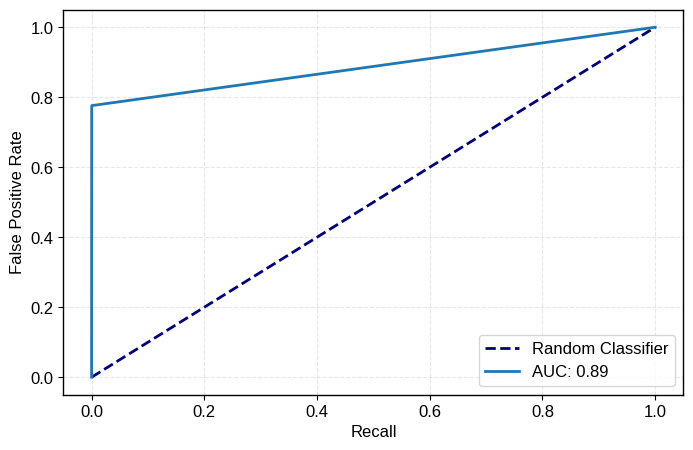
\includegraphics[width=0.7\textwidth]{figuras/modelos_resultados/gru/roc_gru_melhor_fold.png} % insere o tikzpicture puro
  \label{fig:roc_melhor_fold_gru}
  \legend{Fonte: Elaborado pelo autor.}
\end{figure}

Considerando que o \textit{baseline}, um classificador aleatório, tem um \textit{ROC} de 0,5, o melhor foi significantemente melhor.

\begin{figure}[H]
  \centering
  \caption{Curva \textit{ROC} do modelo \ref{fig:gru_pura} em seu melhor \textit{fold}}
   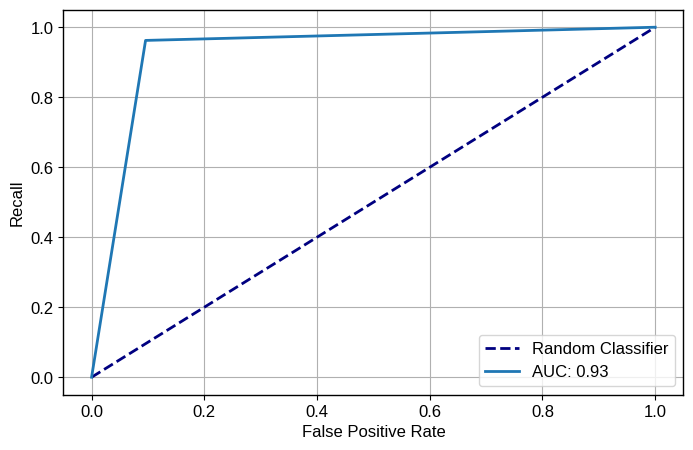
\includegraphics[width=0.7\textwidth]{figuras/modelos_resultados/gru/roc_gru_pior_fold.png} % insere o tikzpicture puro
  \label{fig:roc_pior_fold_gru}
  \legend{Fonte: Elaborado pelo autor.}
\end{figure}

No pior fold, \ref{fig:roc_pior_fold_gru}, o modelo ainda conseguiu manter uma performance satisfatória, com um \textit{ROC} de 0,87. 
Entretanto, devido ao desbalanceamento dos conjuntos, o desempenho pode ser melhor analisado com a curva PR:

\begin{figure}[H]
  \centering
  \caption{Curva precisão vs \textit{recall} do modelo \ref{fig:gru_pura} em seu pior \textit{fold}}
   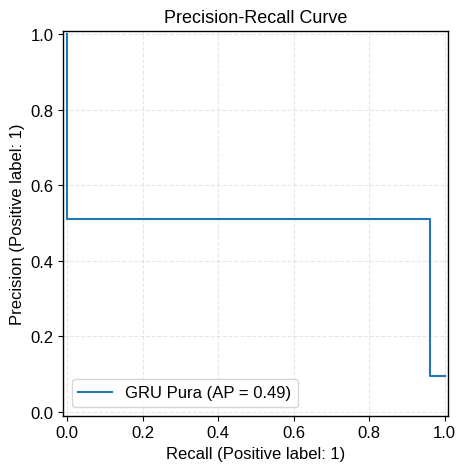
\includegraphics[width=0.7\textwidth]{figuras/modelos_resultados/gru/ap_gru_pior_fold.png} % insere o tikzpicture puro
  \label{fig:ap_gru_pior_fold}
  \legend{Fonte: Elaborado pelo autor.}
\end{figure}

Nesse gráfico, o \textit{baseline} não é fixo, mas igual a prevalência da classe positivos. No pior \textit{fold}, a proporção foi de aproximadamente
9,39\%, contrastando com o 49\% alcançado pelo modelo. Entretanto, a precisão foi baixa. Pelo gráfico, é possível ver que, por exemplo, seria 
possível ter um recall de 80\% porém com uma precisão menor que 60\%.

No melhor caso:

\begin{figure}[H]
  \centering
  \caption{Curva precisão vs \textit{recall} do modelo \ref{fig:gru_pura} em seu melhor \textit{fold}}
   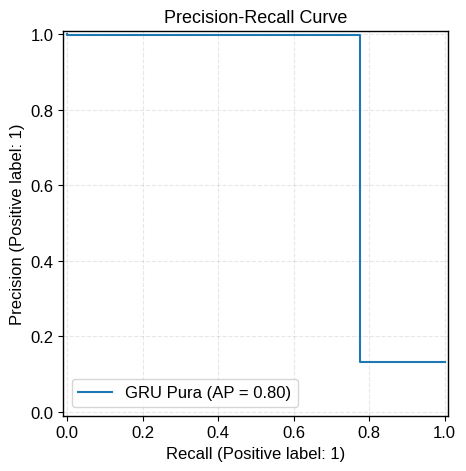
\includegraphics[width=0.7\textwidth]{figuras/modelos_resultados/gru/ap_gru_melhor_fold.png} % insere o tikzpicture puro
  \label{fig:ap_gru_melhor_fold}
  \legend{Fonte: Elaborado pelo autor.}
\end{figure}

Nesse \textit{fold}, o modelo alcançou um \textit{AP} de 80\%, enquanto que a proporção de casos positivos foi de 13,21\%. No melhor caso, 
entretanto, o modelo para ter 80\% de \textit{recall}, teria que baixar sua precisão para menos de 20\%. 

Apesar do desbalanceamento, o modelo alcançou resultados satisfatórios, considerando o extremo desbalanceamento do conjunto.

\section{Resultados do modelo híbrido GRU e CNN}
\label{sec:resultados_gru_cnn}

O modelo híbrido apresentou resultado superior em relação ao modelo descrito em \ref{fig:gru_pura}. Na tabela \ref{tab:resultado_cv_gru_cnn_validacao}
abaixo, é possível ver que o modelo obteve média maior em todas as métricas. Apesar disso, o modelo obteve um desvio padrão maior 
no \textit{recall} e \textit{F1-score}. 

\begin{table}[H]
\centering
\caption{Resultados do modelo híbrido CNN e GRU (\textit{N} vs. \textit{V}) na validação}
\label{tab:resultado_cv_gru_cnn_validacao}
\begin{tabular}{lcc}
\hline
\textbf{Métrica} & \textbf{Média} & \textbf{Desvio Padrão} \\
\hline
Precisão & 0.8800 &  0.1684 \\
\textit{Recall} & 0.8726  & 0.0857 \\
\textit{F1-Score} & 0.8593 & 0.0866 \\
Acurácia & 0.9730 & 0.0258 \\
\hline
\end{tabular}
\legend{Fonte: Elaborado pelo autor.}
\end{table}

Na tabela  \ref{tab:resultado_cv_gru_cnn_treino}, é possível observar que ainda há \textit{overfit} porém a diferença entre os resultados
do treino e validação do modelo \ref{fig:cnn_gru} é menor quando comparado com o modelo \ref{fig:gru_pura}. Por exemplo, a 
diferença percentual entre o \textit{f1-score} do primeiro modelo foi de aproximadamente 9,56\% enquanto que para o segundo, foi de, aproximadamente, 17,98\%

\begin{table}[H]
\centering
\caption{Resultados do modelo híbrido CNN e GRU (\textit{N} vs. \textit{V}) no treino}
\label{tab:resultado_cv_gru_cnn_treino}
\begin{tabular}{lcc}
\hline
\textbf{Métrica} & \textbf{Média} & \textbf{Desvio Padrão} \\
\hline
Precisão & 0.9698 &  0.0180 \\
\textit{Recall} & 0.9313  & 0.0268 \\
\textit{F1-Score} & 0.9502 & 0.0222\\
Acurácia & 0.9915 & 0.0035 \\
\hline
\end{tabular}
\legend{Fonte: Elaborado pelo autor.}
\end{table}

Na figura \ref{fig:gru_cnn_resultados_por_fold}, estão os resultados obtidos pelo modelo híbrido em cada \textit{fold}.

\begin{figure}[H]
  \centering
  \caption{Métricas do modelo híbrido CNN com GRU por \textit{fold}}
   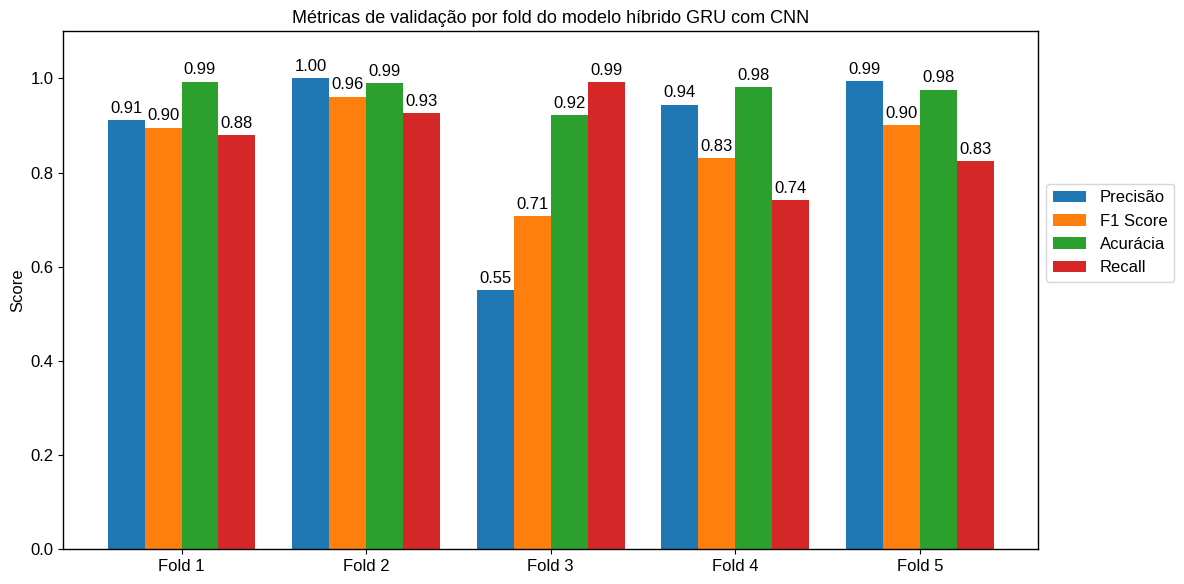
\includegraphics[width=1.0\textwidth]{figuras/modelos_resultados/gru_cnn/gru_cnn_metricas_por_fold.png} 
  \label{fig:gru_cnn_resultados_por_fold}
  \legend{Fonte: Elaborado pelo autor.}
\end{figure}

O modelo manteve a tendencia de ter uma precisão acima da acurácia na maioria dos \textit{folds}. É possível observar também que o modelo
obteve um \textit{recall} maior que o modelo GRU puro em todos os \textit{folds} e uma precisão, no geral, maior ou igual. Sendo as exceções,
os \textit{folds} quatro e cinco, porém a diferença foi de, aproximadamente, 0,01 pontos percentuais. 

A seguir, o desempenho do modelo em seu melhor e pior \textit{fold}. Repetindo os critérios descritos na seção \ref{sec:resultados_gru}, o melhor
\textit{fold} foi o segundo e o pior foi o terceiro.

Na figura \ref{fig:matriz_confusao_cnn_gru_melhor_fold}, é ilustrada a matriz de confusão do modelo em seu melhor \textit{fold}:

\begin{figure}[H]
  \centering
  \caption{Matriz de confusão modelo \ref{fig:cnn_gru} em seu melhor \textit{fold}}
   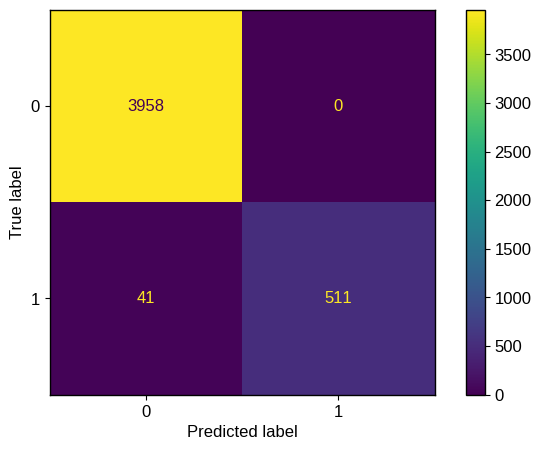
\includegraphics[width=0.7\textwidth]{figuras/modelos_resultados/gru_cnn/matriz_confusao_melhor_fold_gru_cnn_1_alt.png} 
  \label{fig:matriz_confusao_cnn_gru_melhor_fold}
  \legend{Fonte: Elaborado pelo autor.}
\end{figure}

Como pode ser visto no gráfico; o modelo não cometeu nenhum erro de falso positivo e errou 41 arritmias, classificando-as
como batimentos normais. 

Na matriz de confusão do pior \textit{fold}, ilustrado na figura \ref{fig:matriz_confusao_cnn_gru_pior_fold}, novamente,
a situação se inverte; a quantidade de erros de falsos negativos foi menor que as de falsos positivos, refletindo em um
\textit{recall} maior que a precisão; como pode ser observado no gráfico \ref{fig:gru_cnn_resultados_por_fold}.

\begin{figure}[H]
  \centering
  \caption{Matriz de confusão modelo \ref{fig:cnn_gru} em seu melhor \textit{fold}}
   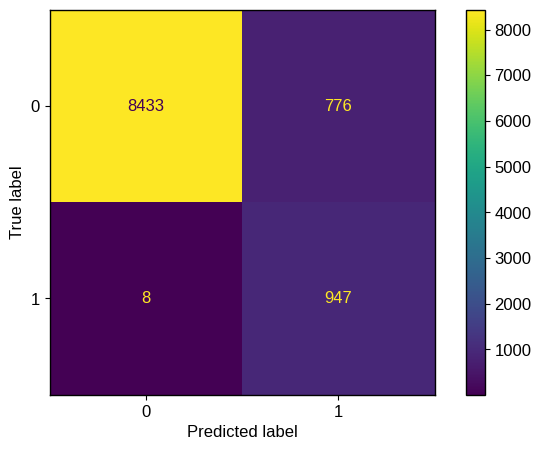
\includegraphics[width=0.7\textwidth]{figuras/modelos_resultados/gru_cnn/matriz_confusao_pior_fold_gru_cnn_3_alt.png} 
  \label{fig:matriz_confusao_cnn_gru_pior_fold}
  \legend{Fonte: Elaborado pelo autor.}
\end{figure}


No melhor, o modelo híbrido obteve um AP de 0,96, como pode ser visto na figura \ref{fig:roc_cnn_gru_melhor_fold}:


\begin{figure}[H]
  \centering
  \caption{Curva \textit{ROC} modelo \ref{fig:cnn_gru} em seu melhor \textit{fold}}
   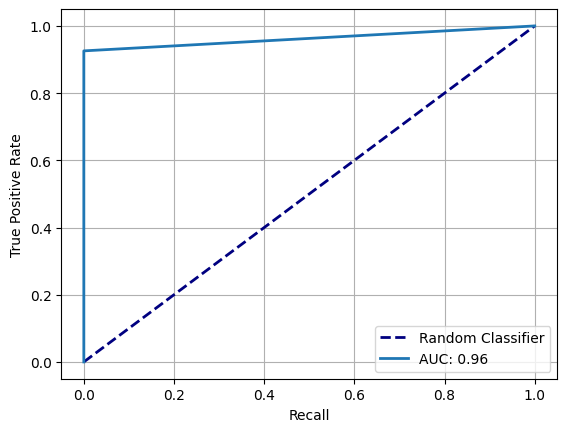
\includegraphics[width=0.7\textwidth]{figuras/modelos_resultados/gru_cnn/roc_cnn_melhor_fold_1.png} 
  \label{fig:roc_cnn_gru_melhor_fold}
  \legend{Fonte: Elaborado pelo autor.}
\end{figure}

Considerando a curva PR, o AP também foi maior:

\begin{figure}[H]
  \centering
  \caption{Curva precisão vs \textit{recall} do modelo \ref{fig:cnn_gru} em seu melhor \textit{fold}}
   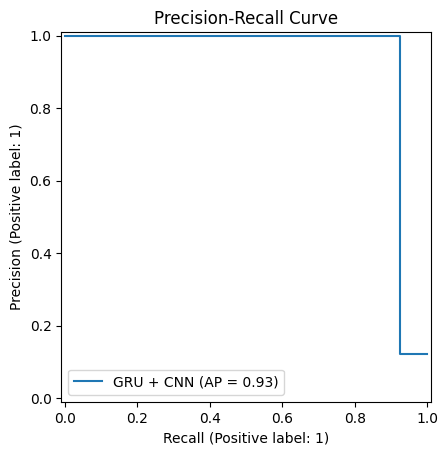
\includegraphics[width=0.7\textwidth]{figuras/modelos_resultados/gru_cnn/ap_gru_cnn_melhor_fold_1.png} 
  \label{fig:ap_cnn_gru_melhor_fold}
  \legend{Fonte: Elaborado pelo autor.}
\end{figure}

Pelo gráfico \ref{fig:ap_cnn_gru_melhor_fold}, nesse \textit{fold}, o modelo conseguiria manter um \textit{recall} de até 80\%
enquanto sua precisão permanece em torno de quase 100\%, desempenho superior ao modelo GRU puro.

A curva \textit{ROC} desse modelo no pior \textit{fold} é descrita a seguir:

\begin{figure}[H]
  \centering
  \caption{Curva \textit{ROC} modelo \ref{fig:cnn_gru} em seu pior \textit{fold}}
   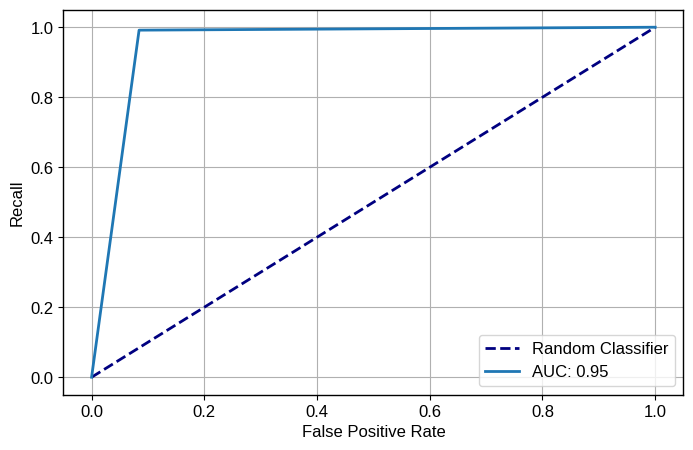
\includegraphics[width=0.7\textwidth]{figuras/modelos_resultados/gru_cnn/roc_cnn_pior_fold_3.png} 
  \label{fig:roc_cnn_gru_pior_fold}
  \legend{Fonte: Elaborado pelo autor.}
\end{figure}

O AP foi de 0,87, igual ao obtido no modelo GRU puro. Já a curva PR descrita na figura

\begin{figure}[H]
  \centering
  \caption{Curva precisão vs \textit{recall} do modelo \ref{fig:cnn_gru} em seu melhor \textit{fold}}
   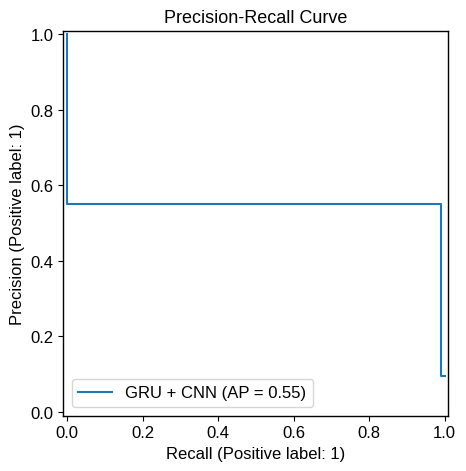
\includegraphics[width=0.7\textwidth]{figuras/modelos_resultados/gru_cnn/ap_gru_cnn_pior_fold_3.png} 
  \label{fig:ap_cnn_gru_pior_fold}
  \legend{Fonte: Elaborado pelo autor.}
\end{figure}

Nesse cenário, o modelo conseguiria manter um \textit{recall} de até 80\% com um pouco menos de 60\% de precisão.

De modo geral, os modelos exibiram um perfil semelhante em seu pior e melhor caso. No pior, a sensibilidade foi maior, resultados
em maiores erros de falso positivo, como resultado, o \textit{recall} foi alto e a precisão foi baixa. No melhor caso, houve um 
equilíbrio maior e, apesar do \textit{recall} mais baixo, a alta precisão aumentou o \textit{f1-score}.

Em contextos médicos, é preferível um \textit{recall} maior, pois falsos negativos são mais danosos que um falso positivo; isto é, é melhor
dizer que um batimento normal é arrítmico do que o contrário. Entretanto, uma precisão muito baixa pode indicar que o modelo é 
tão bom quanto um modelo aleatório; o que o tornaria inútil. 

Como evidenciado pelo AP, ambos os modelos se saíram bem melhor do que esse \textit{baseline}.

\chapter{Análise de erros no pior \textit{fold}}
\label{ch:analise_erros_pior_fold}

Pelos critérios adotados, o pior \textit{fold} de ambos os modelos foi o terceiro. Devido ao \textit{recall} maior que a precisão, supõe-se que 
a razão era por haver batimentos normais com características mais heterodoxas o que pode ter confundido os modelos. Para obter um melhor entendimento
dessa questão, foi feita uma breve análise dos batimentos e pacientes desse \textit{fold}. 

\section{Análise de erros do modelo híbrido CNN com GRU}
\label{sec:analise_erros_cnn_gru}

Na tabela \ref{tab:erros_acertos_por_paciente} a seguir, é possível ver que a maioria dos erros foi oriunda de um paciente, o 203.

\begin{table}[H]
\centering
\caption{Total dos erros e acertos por paciente no \textit{fold} de validação}
\label{tab:erros_acertos_por_paciente}
\begin{tabular}{lcc}
\hline
\textbf{Pacientes} & \textbf{Erros} & \textbf{Acertos}\\
\hline
119 & 0 &  1972 \\
203 & 772  & 2186\\
205 & 11 & 2616\\
209 & 1 & 2606\\
\hline
\end{tabular}
\legend{Fonte: Elaborado pelo autor.}
\end{table}

Aproximadamente, 98,46\% de todos os erros foram desse paciente. O modelo errou em torno de 35,31\% de seus batimentos. Conforme visto na 
figura \ref{fig:matriz_confusao_cnn_gru_pior_fold}, a maioria desses erros são de falsos positivos.

Segundo as anotações do MIT-BIH, disponíveis em \cite{physionet_annotations}, o paciente 203 é considerado como muito difícil. As anotações ainda citam
a presença de mudança de morfologia no complexo QRS e contrações ventriculares prematuras (PVC) de múltiplas formas.